% =====================================================================
% Annexe (page 2) de l'affiche -- Probleme 1, GEI723 (Automne 2026)
% Les deux pages sont reunies dans affiche_complete.pdf par affiche_complete.tex.
% =====================================================================
\documentclass[20pt, a0paper, portrait, margin=0mm, innermargin=24mm,
  colspace=19mm, subcolspace=0mm, blockverticalspace=6mm]{tikzposter}
% =====================================================================
% Style commun de l'affiche et de l'annexe (tikzposter, A0 portrait).
% Compiler avec XeLaTeX (ou LuaLaTeX) : les polices IBM Plex sont dans fonts/.
% =====================================================================
\usepackage{fontspec}
\usepackage{polyglossia}
\setdefaultlanguage{french}
\usepackage{graphicx}
\usepackage{booktabs}
\usepackage{array}
\usepackage{tabularx}
\usepackage{amsmath}
\usepackage{enumitem}
\usetikzlibrary{arrows.meta}

% ---------------------------------------------------------------- polices
\setmainfont{IBMPlexSans}[Path=fonts/, Extension=.ttf, UprightFont=*-Regular,
  BoldFont=*-SemiBold, ItalicFont=*-Italic]
\setsansfont{IBMPlexSans}[Path=fonts/, Extension=.ttf, UprightFont=*-Regular,
  BoldFont=*-SemiBold, ItalicFont=*-Italic]
\setmonofont{IBMPlexMono}[Path=fonts/, Extension=.ttf, UprightFont=*-Regular,
  BoldFont=*-SemiBold]
\newfontfamily\condensed{IBMPlexSansCondensed}[Path=fonts/, Extension=.ttf,
  UprightFont=*-Bold, BoldFont=*-Bold]
\newfontfamily\plexbold{IBMPlexSans}[Path=fonts/, Extension=.ttf, UprightFont=*-Bold]

% ---------------------------------------------------------------- couleurs
\definecolor{encre}{HTML}{16161A}
\definecolor{encre2}{HTML}{2C2C33}
\definecolor{gris}{HTML}{4A4A52}
\definecolor{filet}{HTML}{D9D6CE}
\definecolor{fond}{HTML}{FBFAF7}
\definecolor{carton}{HTML}{FFFFFF}
\definecolor{bordure}{HTML}{E4E2DC}
\definecolor{bleu}{HTML}{2A78D6}
\definecolor{orange}{HTML}{EB6834}
\definecolor{excit}{HTML}{3A3A42}
\definecolor{inhib}{HTML}{C2410C}
\definecolor{ambre}{HTML}{8A6D00}

% ---------------------------------------------------------------- theme tikzposter
\definecolorstyle{Affiche}{}{%
  \colorlet{backgroundcolor}{fond}
  \colorlet{framecolor}{fond}
  \colorlet{titlefgcolor}{encre}
  \colorlet{titlebgcolor}{fond}
  \colorlet{blocktitlebgcolor}{fond}
  \colorlet{blocktitlefgcolor}{encre}
  \colorlet{blockbodybgcolor}{fond}
  \colorlet{blockbodyfgcolor}{encre}
  \colorlet{innerblocktitlebgcolor}{fond}
  \colorlet{innerblocktitlefgcolor}{encre}
  \colorlet{innerblockbodybgcolor}{fond}
  \colorlet{innerblockbodyfgcolor}{encre}
  \colorlet{notefgcolor}{encre}
  \colorlet{notebgcolor}{carton}
  \colorlet{notefrcolor}{bordure}
}
\tikzposterlatexaffectionproofoff
\usecolorstyle{Affiche}
\usebackgroundstyle{Empty}
\usetitlestyle{Empty}
\useblockstyle{Minimal}
\defineblockstyle{Affiche}{titlewidthscale=1, bodywidthscale=1, titleleft,
  titleoffsetx=0pt, titleoffsety=0pt, bodyoffsetx=0pt, bodyoffsety=0pt,
  bodyverticalshift=0pt, roundedcorners=0, linewidth=0pt,
  titleinnersep=0mm, bodyinnersep=0mm}{}
\useblockstyle{Affiche}

% ---------------------------------------------------------------- commandes
% Titre de section numerote : \titre{01}{Contexte et objectifs}
\newcommand{\titre}[2]{{\condensed\fontsize{36pt}{40pt}\selectfont
  {\ttfamily\bfseries\color{bleu}#1}\hspace{0.5em}#2}\par\vspace{3mm}}
% Bandeau de partie, pleine largeur
\newcommand{\bandeau}[1]{\noindent{\ttfamily\bfseries\fontsize{20pt}{24pt}\selectfont\addfontfeature{LetterSpace=8}#1}%
  \hspace{1em}\leaders\hrule height 1.2mm\hfill\null}
% Legende de figure : \legende{Fig. 1 --- Titre.}{Texte}
\newcommand{\legende}[2]{\par\vspace{2mm}{\fontsize{17pt}{23pt}\selectfont\color{encre2}\textbf{#1} #2\par}\vspace{4mm}}
% Numero de piece cercle
\newcommand{\num}[1]{\tikz[baseline=(n.base)]\node[circle, draw=encre, line width=0.4mm, inner sep=0.6mm, font=\fontsize{13pt}{13pt}\selectfont\bfseries] (n) {#1};\ }
% Encadre blanc
\newcommand{\encadre}[1]{\noindent\colorbox{carton}{\fcolorbox{bordure}{carton}{\parbox{\dimexpr\linewidth-2\fboxsep-1.6pt-2\fboxrule\relax}{\raggedright #1}}}}
\newcommand{\code}[1]{\texttt{#1}}
\newcommand{\petit}{\fontsize{18pt}{24.5pt}\selectfont}
\newcommand{\corps}{\fontsize{19.5pt}{27pt}\selectfont}
\setlength{\fboxsep}{5mm}
\setlength{\fboxrule}{0.6mm}
\setlength{\parindent}{0pt}
\setlength{\parskip}{3mm}
\setlist{nosep, leftmargin=0pt, labelsep=0pt, itemsep=3mm}
\renewcommand{\arraystretch}{1.25}
\setlength{\heavyrulewidth}{0.6mm}
\setlength{\lightrulewidth}{0.3mm}

% Schemas TikZ
\tikzset{
  carte/.style={rectangle, rounded corners=1.6mm, line width=0.6mm, align=center, inner sep=1mm},
  pill/.style={rounded corners=8mm},
  etiq/.style={inner sep=0pt, text=gris},
  excitl/.style={draw=excit, line width=0.8mm},
  inhibit/.style={draw=inhib, line width=0.8mm},
  bande/.style={draw=bordure!80!gris, dash pattern=on 3mm off 2.5mm, line width=0.6mm, rounded corners=5mm, fill=bordure!35!fond},
}

% Motif raster du CPG (une barre bleue, une orange, periode 197 ms)
\newcommand{\raster}[1]{%
  \begin{tikzpicture}
    \foreach \i in {0,...,15} {
      \fill[bleu, rounded corners=0.4mm] (\i*5.2,0) rectangle ++(0.19,#1);
      \fill[orange, rounded corners=0.4mm] (\i*5.2+2.6,0) rectangle ++(0.19,#1);
    }
  \end{tikzpicture}}


\renewcommand{\petit}{\fontsize{21pt}{28.5pt}\selectfont}
\renewcommand{\corps}{\fontsize{22pt}{30pt}\selectfont}
\renewcommand{\legende}[2]{\par\vspace{3mm}{\fontsize{20pt}{27pt}\selectfont\color{encre2}\textbf{#1} #2\par}\vspace{6mm}}
\newcommand{\tableparam}[1]{{\fontsize{21pt}{28pt}\selectfont
  \begin{tabularx}{\linewidth}{@{}>{\raggedright\arraybackslash}p{0.25\linewidth} >{\raggedright\arraybackslash}X >{\raggedleft\arraybackslash}p{0.31\linewidth}@{}}
    \toprule \textbf{Élément} & \textbf{Paramètre} & \textbf{Valeur}\\ \midrule
    #1 \bottomrule
  \end{tabularx}}\par}

\begin{document}

\settitle{\begin{minipage}{\linewidth}\raggedright
  {\ttfamily\fontsize{17pt}{20pt}\selectfont\color{gris}
  GEI723 · PROBLÈME 1 · ANNEXE (PAGE 2)\hfill RAPHAËL BARRETTE · ÉMILE JACQUES-TIGHE\par}
  \vspace{6mm}
  {\condensed\fontsize{60pt}{64pt}\selectfont Annexe : paramètres, justifications et expériences complémentaires\par}
  \vspace{6mm}
\end{minipage}}
\maketitle[width=\dimexpr\textwidth-48mm\relax, titletotopverticalspace=20mm, titletoblockverticalspace=12mm, innersep=0mm]

\begin{columns}
\column{0.333}
\block{}{\raggedright%
  \titre{A1}{Paramètres de la Partie I}
  \tableparam{
    Tous & seuil · reset · réfractaire & 1 · 0 · 2 ms\\
    CPG (A, B) & $\tau$ · $\tau_i$ · $\tau_a$ · inc$_a$ & 10 · 20 · 200 ms · 1,5\\
    CPG, départ & $v_0$ · $a_0$ (B part fatigué) & [0,5 ; 0] · [0 ; 1]\\
    Motoneurones & $\tau$ · $\tau_i$ & 2 ms · 10 ms\\
    Interneurones ET & $\tau$ · $\tau_i$ (TAU\_BLOC) & 2 ms · 55 ms\\
    COMPTEUR · INHIB & $\tau$ & 100 s · 2 ms\\
    Poids & W\_AB · W\_MOT · W\_CONTRA · W\_INHIB & 4 · 1,5 · 3 · 3\\
    Porte ET & W\_ET · B\_ET & 0,6 · 0,6\\
    Virage & A → COMPTEUR & 1/n\_saut + 0,01\\
    Délais & CPG → pattes · onde & 3 ms + k$\Delta$\\
  }
  \vspace{3mm}
  {\petit\color{encre2} Durée du blocage : un IN biaisé décharge si $0{,}6 - g_i + 0{,}6 > 1$, soit $g_i < 0{,}2$ ; avec $g_i = 3\,e^{-t/55\,\mathrm{ms}}$, $t = 55 \ln 15 \approx 149$~ms. Le blocage couvre les deux phases d'un cycle de 197~ms et se lève avant le cycle suivant.\par}
  \vspace{16mm}
  \titre{A2}{Paramètres de la Partie II}
  \tableparam{
    Capteurs & M · K · seuils · $\tau$ & 10 · 2 · 0,2→1,8 · 10 ms\\
    Commandes & I\_CMD · W\_WTA · $\tau$ & 1,8 · 1 · 10 ms\\
    Persistance & TAU\_PERSIST · DELAI\_SENS & 800 ms · 0 ms\\
    Mode (CMD → IN) & W\_MODE · G\_MODE · $\tau_s$ des IN & 0,5 · 0,9 · 50 ms\\
    Face & W\_AV\_AR (+) · W\_AV\_AV (−) & 0,05 · 0,04\\
    Flancs & W\_LAT\_CPT · W\_LAT\_AR & 0,04 · 0,025\\
    Compteurs & W\_CPT · TAU\_CPT · W\_AR\_CPT & 0,35 · 150 ms · 3\\
    Arrière & W\_AR\_CPG (lente, vers A et B) & 0,01\\
    Sélection & W\_S\_AV · W\_S\_LAT · W\_S\_GD & 2 · 2 · 1\\
    Habituation & U · $\tau_{\mathrm{rec}}$ & 0,05 · 4 s\\
  }
  \vspace{3mm}
  {\petit\color{encre2} Le biais B\_ET devient un courant lent : chaque décharge de CMD\_AV\_s ($\approx$ 100~Hz) fait $g_s \leftarrow g_s + 0{,}5\,(0{,}9 - g_s)$ sur IN\_sw\_av et IN\_st\_ar. $g_s$ oscille entre $\approx$ 0,63 et 0,76, au-dessus des 0,4 nécessaires ($0{,}6 + g_s > 1$), et retombe en $\approx$ 50~ms quand la commande s'arrête.\par}
  \vspace{3mm}
  {\petit\color{encre2} \textbf{Stimuli.} Un contact injecte K × intensité dans son groupe de capteurs pendant 100~ms. Face : $t_0$ = 1~s, 4~s simulées ; arrière : $t_0$ = 1~s, 3,5~s ; flancs : $t_0$ = 0,5~s, 5~s. Études paramétriques (A7) : $t_0$ = 0,2~s, capteurs, commandes et CPG seulement (sans pattes), sauf la latence ($t_0$ = 1~s, réseau complet).\par}
  \vspace{16mm}
  \titre{A3}{Reproduire}
  \encadre{\ttfamily\fontsize{19pt}{27pt}\selectfont
    pip install -r requirements.txt\\
    python run\_all.py \hfill\# expériences → figures/\\
    python poster\_figs.py \hfill\# figures de l'affiche\\
    python annexe\_figs.py \hfill\# figures de l'annexe\\
    cd affiche \&\& ./build.sh \hfill\# PDF (XeLaTeX)}
}
% ================================================================== colonne 2
\column{0.333}
\block{}{\raggedright%
  \titre{A4}{Capteurs : l'intensité devient un nombre de décharges}
  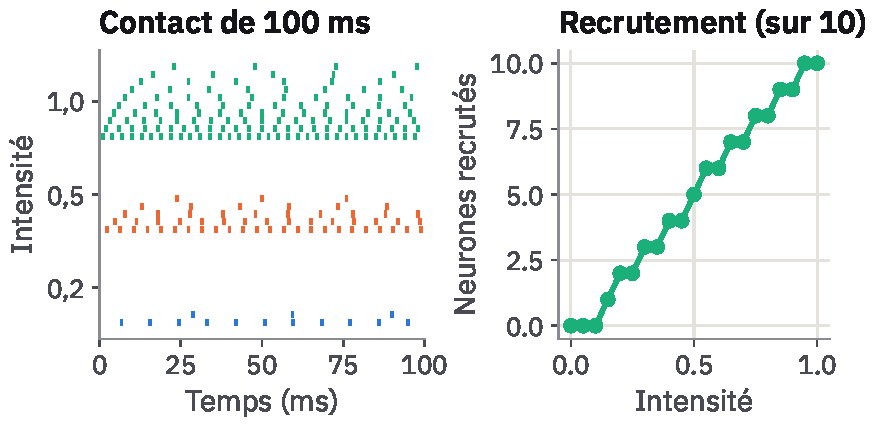
\includegraphics[width=\linewidth]{figures/a_recrutement}
  \legende{Fig. A1 --- Recrutement.}{Les 10 neurones ont des seuils de 0,2 à 1,8 et reçoivent 2 × intensité : un contact faible en fait décharger quelques-uns, lentement ; un contact fort en recrute plus, et plus vite.}
  \vspace{14mm}
  \titre{A5}{Recul selon l'intensité}
  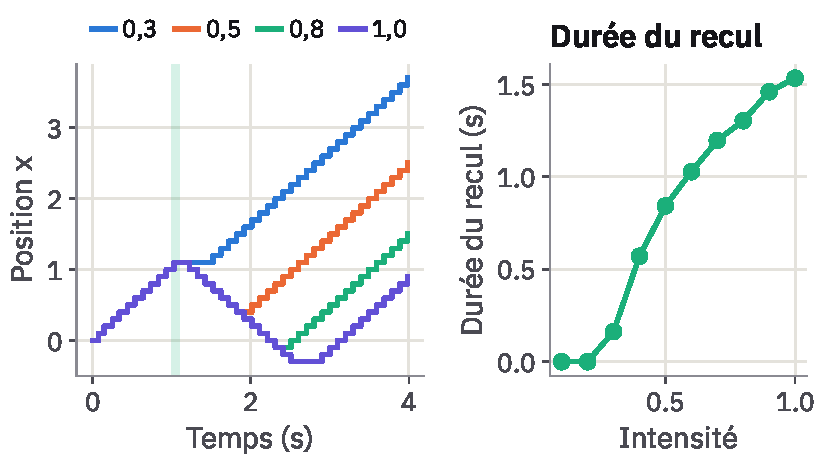
\includegraphics[width=\linewidth]{figures/p2_recul_intensites}
  \legende{Fig. A2 --- Plus l'impact est fort, plus le recul dure.}{Le recul (activité de CMD\_AR\_G) est nul sous 0,3 ; il dure 0,16~s à 0,3, 1,03~s à 0,6 et 1,53~s à 1,0 : le courant lent intègre l'intensité du contact.}
  \vspace{14mm}
  \titre{A6}{Partie II à N paires}
  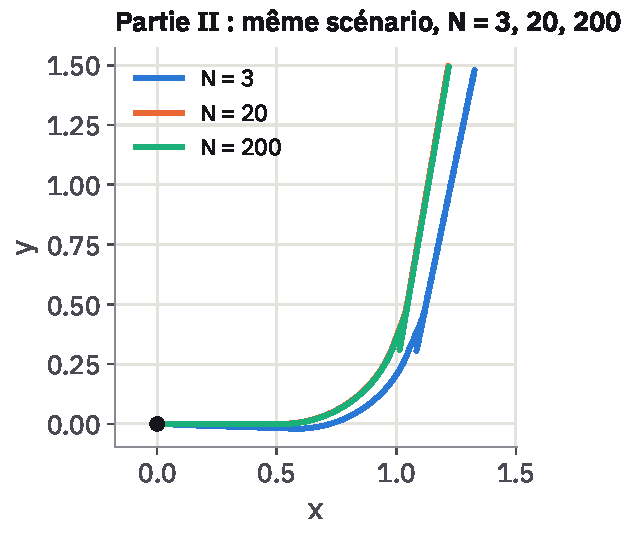
\includegraphics[width=\linewidth]{figures/a_N_partie2}
  \legende{Fig. A3 --- On ne change que N\_PAIRES.}{Contact droit à 0,5~s puis de face à 3~s : capteurs et commandes sont par côté, pas par patte, donc le même réseau de commande pilote 3, 20 ou 200 paires (N = 20 et 200 se superposent).}
}
% ================================================================== colonne 3
\column{0.333}
\block{}{\raggedright%
  \titre{A7}{Adapter le comportement par les paramètres}
  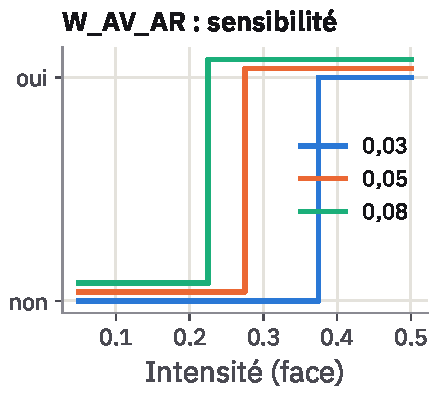
\includegraphics[width=0.49\linewidth]{figures/a_sensibilite}\hfill
  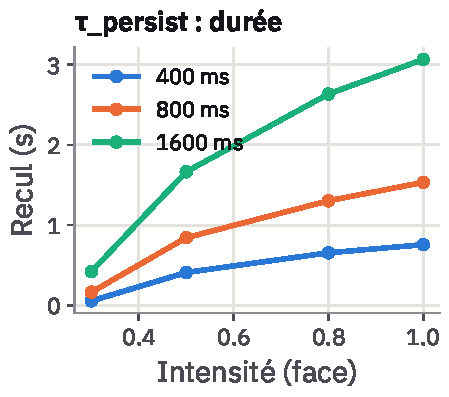
\includegraphics[width=0.49\linewidth]{figures/a_persistance}\par\vspace{3mm}
  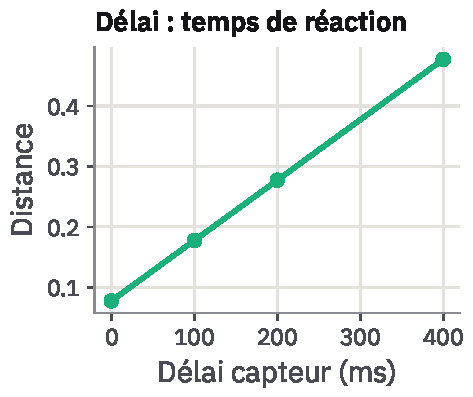
\includegraphics[width=0.49\linewidth]{figures/a_latence}\hfill
  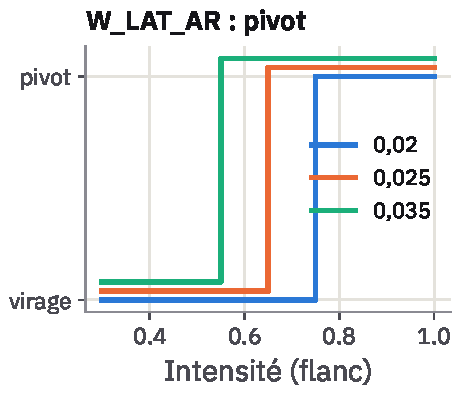
\includegraphics[width=0.49\linewidth]{figures/a_pivot}\par\vspace{3mm}
  \begin{minipage}[c]{0.49\linewidth}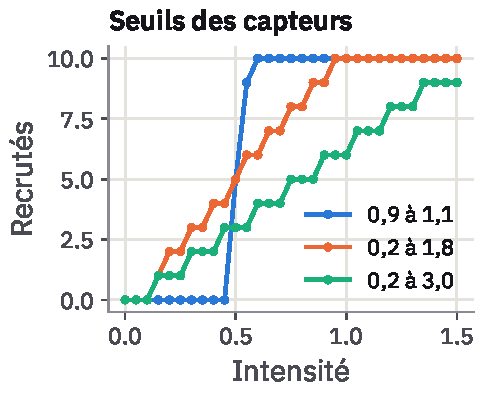
\includegraphics[width=\linewidth]{figures/a_seuils}\end{minipage}\hfill
  \begin{minipage}[c]{0.48\linewidth}\fontsize{18.5pt}{25pt}\selectfont\color{encre2}\raggedright
    \textbf{Fig. A4 --- Un paramètre, un comportement.} W\_AV\_AR = 0,03 → 0,08 abaisse l'intensité minimale de recul de 0,4 à 0,25. Doubler $\tau_{\mathrm{persist}}$ double la durée du recul (0,76 → 1,53 → 3,07~s à l'intensité 1). Chaque 100~ms de délai capteur ajoute $\approx$ 0,1 de distance parcourue avant de reculer. W\_LAT\_AR = 0,02 → 0,035 fait passer le seuil du pivot de 0,8 à 0,6. Des seuils resserrés (0,9 à 1,1) ne distinguent presque plus les intensités.
  \end{minipage}
  \vspace{16mm}
  \titre{A8}{Pourquoi quatre interneurones ?}
  {\corps Sans IN, AVANT recevrait le swing (poids $w_{sw}$), le stance ($w_{st}$) et un biais $b$ qui dépend du mode. Il faudrait :\par}
  \vspace{3mm}
  {\fontsize{22pt}{29pt}\selectfont
  \begin{tabularx}{\linewidth}{@{}l X X@{}}
    \toprule \textbf{Mode} & \textbf{Swing → AVANT} & \textbf{Stance → AVANT}\\ \midrule
    avant & $w_{sw} + b_{av} > 1$ & $w_{st} + b_{av} < 1$\\
    arrière & $w_{sw} + b_{ar} < 1$ & $w_{st} + b_{ar} > 1$\\ \bottomrule
  \end{tabularx}\par}
  \vspace{3mm}
  {\corps La colonne swing impose $b_{av} > b_{ar}$, la colonne stance $b_{ar} > b_{av}$ : contradiction. AVANT calcule un XNOR (phase, mode), non linéairement séparable ; il faut une couche cachée. Chaque IN fait un ET, AVANT et ARRIÈRE font le OU de deux IN. Choisir la source d'AVANT en Python marcherait aussi, mais le mode deviendrait un recâblage au lieu d'un signal.\par}
}
\end{columns}

\end{document}
